\documentclass[10pt,xcolor={x11names}]{beamer}

\usetheme[numbering=fraction,block=fill]{metropolis}
\usecolortheme{seahorse}
\setbeamertemplate{blocks}[rounded]

\usepackage{kmath}
% Tikz
\usetikzlibrary{calc}
\usetikzlibrary{mindmap,trees,shapes,arrows,backgrounds,topaths}
\usetikzlibrary{decorations.pathmorphing, shapes.geometric}

% Text
\usepackage{enumitem}
\usepackage{ulem}
\usepackage{pifont}

% Maths
\usepackage{amsmath}
\usepackage{amsfonts}
\usepackage{amsthm}
\usepackage{amsopn}

% Plots
\usepackage{pgfplots}
\usepgfplotslibrary{groupplots}

% Tables
\usepackage{booktabs}
\usepackage{array}
\newcolumntype{L}{>$l<$}
\arraycolsep=1.4pt
\setlength{\tabcolsep}{3pt}

% Algos
\usepackage[ruled]{algorithm2e}

% Pgfplot
\pgfplotsset{
    legend image code/.code={
        \draw[mark repeat=2,mark phase=2] plot coordinates {
            (0cm,0cm)
            (0.25cm,0cm)
            (0.25cm,0cm)
        };
    }
}
% Objective values and functions
\newcommand{\pobj}{p}
\newcommand{\robj}{r}
\newcommand{\dobj}{d}

% Variables
\newcommand{\pvletter}{x}
\newcommand{\wvletter}{w}
\newcommand{\dvletter}{u}
\newcommand{\vvletter}{v}
\newcommand{\bvletter}{z}
\newcommand{\pv}{\mathbf{\pvletter}}
\newcommand{\wv}{\mathbf{\wvletter}}
\newcommand{\dv}{\mathbf{\dvletter}}
\newcommand{\vv}{\mathbf{\vvletter}}
\newcommand{\bv}{\mathbf{\bvletter}}
\newcommand{\pvi}[1]{\pvletter_{#1}}
\newcommand{\wvi}[1]{\wvletter_{#1}}
\newcommand{\dvi}[1]{\dvletter_{#1}}
\newcommand{\vvi}[1]{\vvletter_{#1}}
\newcommand{\bvi}[1]{\bvletter_{#1}}

% Problem data
\newcommand{\pdim}{n}
\newcommand{\ddim}{m}
\newcommand{\dic}{\mathbf{A}}
\newcommand{\dici}[1]{\mathbf{a}_{#1}}
\newcommand{\dicii}[1]{a_{#1}}
\newcommand{\obs}{\mathbf{y}}
\newcommand{\obsi}[1]{y_{#1}}
\newcommand{\reg}{\lambda}
\newcommand{\groundtruth}{\pv^{\dagger}}
\newcommand{\lfunc}{f}
\newcommand{\pfunc}{h}
\newcommand{\rfunc}{g}
\newcommand{\dfunc}{D}
\newcommand{\relaxrfunc}{\tilde{g}}
\newcommand{\relaxpfunc}{\tilde{h}}
\newcommand{\bigM}{M}
\newcommand{\regtwo}{\alpha}
\newcommand{\rslope}{\tau}
\newcommand{\rlimit}{\mu}
\newcommand{\noise}{\boldsymbol{\epsilon}}

% Indices
\newcommand{\idxentry}{i}

% BnB
\newcommand{\pset}{\mathcal{X}}
\newcommand{\setidx}{\mathcal{S}}
\newcommand{\setzero}{\setidx_0}
\newcommand{\setone}{\setidx_1}
\newcommand{\setnone}{\setidx_\bullet}
\newcommand{\nodeSymb}{\nu}
\newcommand{\node}[1]{#1^{\nodeSymb}}

% Screening
\newcommand{\saferegion}{\mathcal{R}}
\newcommand{\safesphere}{\mathcal{S}}
\newcommand{\spherecenter}{\mathbf{c}}
\newcommand{\sphereradius}{r}

% Peeling
\newcommand{\bigL}{\boldsymbol{\alpha}}
\newcommand{\bigU}{\boldsymbol{\beta}}
\newcommand{\bigLi}[1]{\alpha_{#1}}
\newcommand{\bigUi}[1]{\beta_{#1}}

% Math operators
\DeclareMathOperator{\argmax}{argmax}
\DeclareMathOperator{\argmin}{argmin}
\DeclareMathOperator{\biconjugate}{biconj}
\DeclareMathOperator{\card}{card}
\DeclareMathOperator{\complset}{cmpl}
\DeclareMathOperator{\convex}{cvx}
\DeclareMathOperator{\diam}{diam}
\DeclareMathOperator{\dom}{dom}
\DeclareMathOperator{\interior}{int}
\DeclareMathOperator{\prox}{prox}
\DeclareMathOperator{\rank}{rank}
\DeclareMathOperator{\sign}{sign}


% Math misc
\newcommand{\1}{\mathbf{1}}
\newcommand{\0}{\mathbf{0}}
\newcommand{\abs}[1]{|#1|}
\newcommand{\biconj}[1]{#1^{**}}
\newcommand{\bigO}{\mathcal{O}}
\newcommand{\conj}[1]{#1^{*}}
\newcommand{\icvx}{\eta}
\newcommand{\intervint}[2]{[#1,#2]}
\newcommand{\iter}[2]{#1^{#2}}
\newcommand{\norm}[2]{\|#1\|_#2}
\newcommand{\opt}[1]{#1^{\star}}
\newcommand{\pospart}[1]{[#1]_+}
\newcommand{\separable}[2]{#1_{#2}}
\newcommand{\subdiff}{\partial}
\newcommand{\transp}[1]{#1^{\mathrm{T}}}

% Edition macros
\newcommand{\AddTodo}[1]{\textcolor{red}{[#1]}}

\tikzset{
  invisible/.style={opacity=0},
  visible on/.style={alt={#1{}{invisible}}},
  alt/.code args={<#1>#2#3}{%
    \alt<#1>{\pgfkeysalso{#2}}{\pgfkeysalso{#3}} % \pgfkeysalso doesn't change the path
  },
}

\newenvironment<>{blockzero}[1]{%
  \begin{block}#2{\centering#1\par}}{\end{block}}
\newenvironment<>{blockone}[1]{%
  \setbeamercolor{block title}{fg=mLightGreen,bg=mLightGreen!20}%
  \setbeamercolor{block body}{fg=mLightGreen,bg=mLightGreen!20}%
  \begin{block}#2{\centering#1\par}}{\end{block}}
\newenvironment<>{blocktwo}[1]{%
  \setbeamercolor{block title}{fg=mLightBrown,bg=mLightBrown!20}%
  \setbeamercolor{block body}{fg=mLightBrown,bg=mLightBrown!20}%
  \begin{block}#2{\centering#1\par}}{\end{block}}
\newenvironment<>{blockthree}[1]{%
  \setbeamercolor{block title}{fg=purple,bg=purple!20}%
  \setbeamercolor{block body}{fg=purple,bg=purple!20}%
  \begin{block}#2{\centering#1\par}}{\end{block}}
\newenvironment<>{blockfour}[1]{%
  \setbeamercolor{block title}{fg=blue,bg=blue!20}%
  \setbeamercolor{block body}{fg=blue,bg=blue!20}%
  \begin{block}#2{\centering#1\par}}{\end{block}}
\newenvironment<>{blockfive}[1]{%
  \setbeamercolor{block title}{fg=blue,bg=blue!30}%
  \setbeamercolor{block body}{fg=blue,bg=blue!20}%
  \begin{block}#2{\centering#1\par}}{\end{block}}
\newenvironment<>{blocksix}[1]{%
  \setbeamercolor{block title}{fg=black,bg=black!16}%
  \setbeamercolor{block body}{fg=black,bg=black!16}%
  \begin{block}#2{\centering#1\par}}{\end{block}}
\newenvironment<>{blockseven}[1]{%
  \setbeamercolor{block title}{fg=black,bg=white}%
  \setbeamercolor{block body}{fg=black,bg=white}%
  \begin{block}#2{\centering#1\par}}{\end{block}}

\newcommand{\emphone}[1]{{\color{mLightGreen}#1}}
\newcommand{\emphtwo}[1]{{\color{mLightBrown}#1}}
\newcommand{\emphthree}[1]{{\color{purple}#1}}
\newcommand{\emphfour}[1]{{\color{blue}#1}}

\title{Unifying Branch-and-Bound Approaches to Solve L0-Penalized Problems}
\date{Inria Rennes, France}
\author{\textbf{Theo Guyard} with C. Herzet, A. Arslan and C. Elvira}
\institute{SIAM Conference on Optimization \\ Seattle, USA \\ 2023}


\begin{document}

\maketitle

\section{L0-penalized problems}

\begin{frame}{Sparse optimization}
    \begin{tikzpicture}[remember picture,overlay]
        \onslide<+-> {
            \draw [ultra thick,<->] ($(current page.north)+(-2.2,-0.32\textheight)$) -- ($(current page.north)+(2.2,-0.32\textheight)$) node (arrow) [midway] {};
            \node at ($(arrow.north)+(0,0.1)$) {\textbf{Sparse optimization}};
            \node [text width=0.3\textwidth] at ($(current page.north)+(-4,-0.3\textheight)$) (obs) {
                \begin{blockone}{}
                    \centering
                    \textbf{Minimize a loss}
                \end{blockone}
            };
            \node [text width=.3\textwidth] at ($(current page.north)+(4,-0.3\textheight)$) (dic) {
                \begin{blocktwo}{}
                    \centering
                    \textbf{Sparse solution}
                \end{blocktwo}
            };
            \node at ($(arrow.south)+(0,-0.6)$) (applications) {
                \begin{varwidth}{\linewidth}
                    \centering
                    \scriptsize{Machine Learning} \\
                    \scriptsize{Signal processing} \\
                    \scriptsize{Network design} \\
                    \scriptsize{...}
                \end{varwidth}
            };
        };
        %
        %
        %
        \onslide<+-> {
            \node [text width=.45\textwidth] at ($(current page.north)+(0,-0.6\textheight)$) (problem) {
                \begin{blockthree}{$\ell_0$-penalized problem}
                    \centering
                    $\min_{\pv} \ \datafunc(\pv) + \reg \norm{\pv}{0} + \regfunc(\pv)$
                \end{blockthree}
            };
            \node [text width=.45\textwidth] at ($(current page.north)+(1.5,-0.82\textheight)$) (problem) {
                \begin{itemize}[nosep]
                    \item[$\datafunc(\cdot)$]: loss
                    \item[$\norm{\cdot}{0}$]: sparsity
                    \item[$\reg$]: trade-off
                    \item[$\regfunc(\cdot)$]: modelling
                \end{itemize}
            };
        }
    \end{tikzpicture}
\end{frame}

\begin{frame}{Contributions}
    \begin{tikzpicture}[remember picture,overlay]
        \onslide {
            \node<+-> [text width=.45\textwidth] at ($(current page.north)+(0,-0.25\textheight)$) (problem) {
                \begin{blockthree}{L0-penalized problem}
                \centering
                $\min_{\pv} \ \datafunc(\pv) + \reg \norm{\pv}{0} + \regfunc(\pv)$
                \end{blockthree}
            };
            \node at ($(problem.south)+(0,-0.2)$) (problem) {\textbf{NP-hard}};
        }
        \node<+-> [text width=.3\textwidth, anchor=north] at ($(problem.south)+(-4,-0.4)$) (mip) {
            \begin{blockzero}{Generic approaches}
            \centering
            \scriptsize
            ~\\
            \begin{itemize}[leftmargin=*,label=$\blacktriangleright$,nosep]
                \item D. Bertsimas \hfill (2016)
                \item S. Bourguignon \hfill (2017)
                \item A. Atamtürk \hfill (2020)
                \item D. Bertsimas \hfill (2021)
                \item C. Kanzow \hfill (2022)
                \item ...
            \end{itemize}
            ~\\
            \emphone{
                \begin{itemize}[leftmargin=*,label=\ding{51},nosep]
                    \item Off-the-shelf MIP solver
                \end{itemize}
            }
            \emphtwo{
                \begin{itemize}[leftmargin=*,label=\ding{55},nosep]
                    \item Slow
                \end{itemize}
            }
            \emphone{
                \begin{itemize}[leftmargin=*,label=\ding{51},nosep]
                    \item Arbitrary $\datafunc(\cdot)$ and $\regfunc(\cdot)$
                \end{itemize}
            }
            \end{blockzero}
        };
        \node<+-> [text width=.3\textwidth, anchor=north] at ($(problem.south)+(0,-0.4)$) (bnb) {
            \begin{blockzero}{Tailored approaches}
            \centering
            \scriptsize
            ~\\
            \begin{itemize}[leftmargin=*,label=$\blacktriangleright$,nosep]
                \item R. Ben Mhenni \hfill (2021)
                \item H. Hazimeh \hfill (2021)
                \item G. Samain \hfill (2022)
                \item A. Olama \hfill (2022)
                \item A. Atamtürk \hfill (2022)
                \item ...
            \end{itemize}
            ~\\
            \emphone{
                \begin{itemize}[leftmargin=*,label=\ding{51},nosep]
                    \item Branch-and-Bound
                \end{itemize}
            }
            \emphone{
                \begin{itemize}[leftmargin=*,label=\ding{51},nosep]
                    \item Fast
                \end{itemize}
            }
            \emphtwo{
                \begin{itemize}[leftmargin=*,label=\ding{55},nosep]
                    \item Specific $\datafunc(\cdot)$ and $\regfunc(\cdot)$
                \end{itemize}
            }
            \end{blockzero}
        };
        \node<+-> [text width=.3\textwidth, anchor=north] at ($(problem.south)+(4,-0.4)$) (contrib) {
            \begin{blockzero}{Contribution}
            \centering
            \scriptsize
            ~\\
            \begin{itemize}[leftmargin=*,label=$\blacktriangleright$,nosep]
                \item This talk \hfill (2023)
                \item Extended paper \hfill (202?)
            \end{itemize}
            \begin{itemize}[leftmargin=*,nosep]
                \item 
                \item 
                \item
                \item
            \end{itemize}
            ~\\
            \emphone{
                \begin{itemize}[leftmargin=*,label=\ding{51},nosep]
                    \item Branch-and-Bound
                \end{itemize}
            }
            \emphone{
                \begin{itemize}[leftmargin=*,label=\ding{51},nosep]
                    \item Fast
                \end{itemize}
            }
            \emphone{
                \begin{itemize}[leftmargin=*,label=\ding{51},nosep]
                    \item Arbitrary $\datafunc(\cdot)$ and $\regfunc(\cdot)$
                \end{itemize}
            }
            \end{blockzero}
        };
    \end{tikzpicture}
\end{frame}
  
\section{Branch-and-Bound}

\begin{frame}{Algorithmic concept}
    \begin{tikzpicture}[remember picture,overlay]
        \onslide<+-> {
            \node (concept) at ($(current page.north)+(0,-0.2\textwidth)$) {\textit{``Enumerate all candidate solutions and discard sub-optimal ones.''}};
        }
        %
        %
        %
        \onslide<+-> {
            \node (path0) at ($(current page.north)+(1.5,-3.5)$) {};
            \node (path1) at ($(path0)+(2,0)$) {};
            \node (path2) at ($(path0)+(3,-1)$) {};
            \node (path3) at ($(path0)+(2,-3)$) {};
            \node (path4) at ($(path0)+(1,-1.5)$) {};
            \node (path5) at ($(path0)+(0,-1)$) {};
            \path[ultra thick,draw,use Hobby shortcut,closed=true] (path0)..(path1)..(path2)..(path3)..(path4)..(path5);
        }
        %
        %
        %
        \onslide<+-> {
            \draw[ultra thick,dashed] (path2) -- (path4);
        }
        %
        %
        %
        \onslide<+-> {
            \draw[ultra thick,dashed] ($(path4)+(0.75,0.2)$)-- ($(path1)+(-1,0.4)$);
            \draw[ultra thick,dashed] ($(path4)+(1,0.2)$) -- ($(path3)+(0.5,0)$);
        }
        %
        %
        %
        \onslide<+-> {
            \node (N5cross) at ($(path0)+(1.75,-2)$) {\textcolor{purple}{\LARGE\ding{55}}}; 
            \node (N6cross) at ($(path0)+(2.75,-2)$) {\textcolor{purple}{\LARGE\ding{55}}}; 
        }
        %
        %
        %
        \onslide<+-> {
            \node[text width=\textwidth] (principles1) at ($(current page.north)+(2,-0.65\textwidth)$) {
                \textbf{\hspace*{-1.5cm}Main principles}
                \begin{itemize}
                    \item[Branching:] Divide the search space
                    \item[Bounding:] Test whether a region can contain optimal solutions 
                    \item[Pruning:] Discard regions without optimal solutions
                \end{itemize}
            };
        }
    \end{tikzpicture}        
\end{frame}

\begin{frame}{Tree exploration}
    \begin{tikzpicture}[remember picture,overlay]
        \onslide<+-> {
            \node at ($(current page.north)+(0,-0.35\textheight)$) (node0) {};
            \draw[
                ultra thick,
                top color = white,
                bottom color = blue!30,
            ] (node0) circle (15pt) node {\Large$N_0$};
        }
        %
        %
        %
        \onslide<+-> {
            \node at ($(node0)+(-2,-1.5)$) (node1) {};
            \draw[
                ultra thick,
                top color = white,
                bottom color = blue!30,
            ] (node1) circle (15pt) node {\Large$N_1$};
            \draw[ultra thick,->] ($(node0.south west)+(-0.25,-0.25)$) -- ($(node1.north east)+(0.25,0.25)$);
            %
            \node at ($(node0)+(2,-1.5)$) (node2) {};
            \draw[
                ultra thick,
                top color = white,
                bottom color = blue!30,
            ] (node2) circle (15pt) node {\Large$N_2$};
            \draw[ultra thick,->] ($(node0.south east)+(0.25,-0.25)$) -- ($(node2.north west)+(-0.25,0.25)$);
        }
        %
        %
        %
        \onslide<+-> {
            \node (arrowcenter) at ($(node0)+(0,-5)$) {};
            \draw[ultra thick,->] ($(arrowcenter)+(-5,0)$) -- ($(arrowcenter)+(5,0)$) node [above left, xshift=-2pt] {\small{value}};
            \draw[fill] (arrowcenter) circle (2pt) node[below] (popt) {opt.};
        }
        %
        %
        %
        \onslide<+-> {
            \draw[fill,mLightBrown] ($(arrowcenter)+(1.5,0)$) circle (2pt) node (pub1) {};
            \node<-4> [above] (pub1text) at (pub1) {\emphtwo{$\UB{\pobj}_1$}};
            %
            \draw[fill,mLightGreen] ($(arrowcenter)+(-2,0)$) circle (2pt) node (plb1) {};
            \node<-4> [below] (plb1text) at (plb1) {\emphone{$\LB{\pobj}_1$}};
            %
            \draw[fill,mLightBrown] ($(arrowcenter)+(2,0)$) circle (2pt) node  (pub2) {};
            \node<-4> [above] (pub2text) at (pub2) {\emphtwo{$\UB{\pobj}_2$}};
            %
            \draw[fill,mLightGreen] ($(arrowcenter)+(0.75,0)$) circle (2pt) node (plb2) {};
            \node<-4> [below] (plb2text) at (plb2) {\emphone{$\LB{\pobj}_2$}};
        }
        %
        %
        %
        \onslide<+-> {
            \node at ($(node1)+(-1,-1.5)$) (node3) {};
            \draw[
                ultra thick,
                top color = white,
                bottom color = blue!30,
            ] (node3) circle (15pt) node {\Large$N_3$};
            \draw[ultra thick,->] ($(node1.south west)+(-0.25,-0.25)$) -- ($(node3.north)+(0.25,0.35)$);
            \draw[ultra thick,->] ($(node3.south east)+(0.25,-0.25)$) -- ($(node3.south east)+(0.5,-0.5)$);
            \draw[ultra thick,->] ($(node3.south west)+(-0.25,-0.25)$) -- ($(node3.south west)+(-0.5,-0.5)$);
            %
            \node at ($(node1)+(1,-1.5)$) (node4) {};
            \draw[
                ultra thick,
                top color = white,
                bottom color = blue!30,
            ] (node4) circle (15pt) node {\Large$N_4$};
            \draw[ultra thick,->] ($(node1.south east)+(0.25,-0.25)$) -- ($(node4.north)+(-0.25,0.35)$);
            \draw[ultra thick,->] ($(node4.south east)+(0.25,-0.25)$) -- ($(node4.south east)+(0.5,-0.5)$);
            \draw[ultra thick,->] ($(node4.south west)+(-0.25,-0.25)$) -- ($(node4.south west)+(-0.5,-0.5)$);
        }
        %
        %
        %
        \onslide<+-> {
            \draw[fill,mLightBrown] ($(arrowcenter)+(1,0)$) circle (2pt) node (pub3) {};
            \node<-6> [above] (pub3text) at (pub3) {\emphtwo{$\UB{\pobj}_3$}};
            %
            \draw[fill,mLightGreen] ($(arrowcenter)+(-1,0)$) circle (2pt) node (plb3) {};
            \node<-6> [below] (plb3text) at (plb3) {\emphone{$\LB{\pobj}_3$}};
            %
            \draw[fill,mLightBrown] ($(arrowcenter)+(3,0)$) circle (2pt) node (pub4) {};
            \node<-6> [above] (pub4text) at (pub4) {\emphtwo{$\UB{\pobj}_4$}};
            %
            \draw[fill,mLightGreen] ($(arrowcenter)+(-3,0)$) circle (2pt) node (plb4) {};
            \node<-6> [below] (plb5text) at (plb4) {\emphone{$\LB{\pobj}_4$}};
        }
        %
        %
        %
        \onslide<+-> {
            \node at ($(node2)+(-1,-1.5)$) (node5) {};
            \draw[
                ultra thick,
                top color = white,
                bottom color = blue!30,
            ] (node5) circle (15pt) node {\Large$N_5$};
            \draw[ultra thick,->] ($(node2.south west)+(-0.25,-0.25)$) -- ($(node5.north)+(0.25,0.35)$);
            \node at ($(node2)+(1,-1.5)$) (node6) {};
            \draw[
                ultra thick,
                top color = white,
                bottom color = blue!30,
            ] (node6) circle (15pt) node {\Large$N_6$};
            \draw[ultra thick,->] ($(node2.south east)+(0.25,-0.25)$) -- ($(node6.north)+(-0.25,0.35)$);
        }
        %
        %
        %
        \onslide<+-> {
            \draw[fill,mLightGreen] ($(arrowcenter)+(1.75,0)$) circle (2pt) node[below] (plb5) {\emphone{$\LB{\pobj}_5$}};
            \draw[fill,mLightGreen] ($(arrowcenter)+(2.75,0)$) circle (2pt) node[below] (plb6) {\emphone{$\LB{\pobj}_6$}};
            \draw[ultra thick,<-,mLightBrown] ($(pub3)+(0,0.15)$) -- ($(pub3)+(0,0.6)$) node[above] {\small{Best UB}};
        }
        %
        %
        %
        \onslide<+-> {
            \draw[ultra thick,-{Circle[scale=0.5]}] ($(node5.south)+(0,-0.4)$) -- ($(node5.south)+(0,-0.6)$);
            \draw[ultra thick,-{Circle[scale=0.5]}] ($(node6.south)+(0,-0.4)$) -- ($(node6.south)+(0,-0.6)$);
        }
        %
        %
        %
        \onslide<+-> {
            \node[align=center] (convcrit1) at ($(current page.north)+(4,-2)$) {\small{All nodes explored}};
            \node[align=center] (convcrit2) at ($(convcrit1)+(0,-0.3)$) {\small{or pruned}};
            \node[align=center] (convres) at ($(convcrit2)+(0,-1)$) {\small{Problem solved}};
            \draw[ultra thick,->] (convcrit2) -- (convres);
        }
    \end{tikzpicture}
\end{frame}

\begin{frame}{Ingredients}
    \begin{tikzpicture}[remember picture,overlay]
        \node [text width=.45\textwidth] at ($(current page.north)+(0,-0.3\textheight)$) (problem) {
            \begin{blockthree}{$\ell_0$-penalized problem}
                \centering
                $\min_{\pv} \ \datafunc(\pv) + \reg \norm{\pv}{0} + \regfunc(\pv)$
            \end{blockthree}
        };
        \node [text width=\textwidth] at ($(current page.north)+(0,-0.65\textheight)$) (observations) {
            \textbf{What do we need}
            \begin{itemize}[label=$\blacktriangleright $]
                \item A \emphtwo{branching} strategy
                \item A \emphtwo{bounding} strategy
                \item Something \emphtwo{generic} with respect to $\datafunc(\cdot)$ and $\regfunc(\cdot)$
            \end{itemize}
        };
    \end{tikzpicture}
\end{frame}
\section{Generic solution method}

\begin{frame}{Branching}
    \begin{tikzpicture}[remember picture,overlay]
        \onslide<+-> {
            \node at ($(current page.north)+(0,-0.35\textheight)$) (parent) {};
            \draw[
                ultra thick,
                top color = white,
                bottom color = blue!30,
            ] (parent) circle (15pt) node {\Large$\nodeSymbIter{}$};
            \draw[ultra thick,->] ($(parent.north)+(0,0.75)$) -- ($(parent.north)+(0,0.4)$);
            \node at ($(parent)+(0,1.25)$) (branchingrule) {\textbf{Force the (non-)nullity of an entry}};
        }
        %
        %
        %
        \onslide<+-> {
            \node at ($(parent)+(-2,-2)$) (child0) {};
            \draw[
                ultra thick,
                top color = white,
                bottom color = blue!30,
            ] (child0) circle (15pt) node {\Large$\nodeSymbIter{}_0$};
            \draw[ultra thick,->] ($(parent.south west)+(-0.25,-0.25)$) -- ($(child0.north east)+(0.25,0.25)$) node[midway,draw,fill=white] {$\pvi{\idxentry} = 0$};
            \node at ($(parent)+(2,-2)$) (child1) {};
            \draw[
                ultra thick,
                top color = white,
                bottom color = blue!30,
            ] (child1) circle (15pt) node {\Large$\nodeSymbIter{}_1$};
            \draw[ultra thick,->] ($(parent.south east)+(0.25,-0.25)$) -- ($(child1.north west)+(-0.25,0.25)$) node[midway,draw,fill=white] {$\pvi{\idxentry} \neq 0$};
            \draw[ultra thick,->] ($(child0.south west)+(-0.25,-0.25)$) -- ($(child0.south west)+(-0.5,-0.5)$);
            \draw[ultra thick,->] ($(child0.south east)+(0.25,-0.25)$) -- ($(child0.south east)+(0.5,-0.5)$);
            \draw[ultra thick,->] ($(child1.south west)+(-0.25,-0.25)$) -- ($(child1.south west)+(-0.5,-0.5)$);
            \draw[ultra thick,->] ($(child1.south east)+(0.25,-0.25)$) -- ($(child1.south east)+(0.5,-0.5)$);
        }
        %
        %
        %
        \onslide<+-> {
            \node at ($(parent)+(1.25,0)$) (parentsets) {$(\setzero,\setone)$};
        }
        %
        %
        %
        \onslide<+-> {
            \node at ($(child0)+(-1.75,0)$) (child0sets) {$(\setzero\emphtwo{\cup\{\idxentry\}},\setone)$};
            \node at ($(child1)+(1.75,0)$) (child1sets) {$(\setzero,\setone\emphtwo{\cup\{\idxentry\}})$};
        }
        %
        %
        %
        \onslide<+-> {
            \node[text width=.5\textwidth] at ($(current page.north)+(0,-0.85\textheight)$) (nodeproblem) {
                \begin{blockthree}{Node problem}
                    \centering
                    \small
                    $
                        \left\{
                        \begin{array}{rl}
                            \min_{\pv} & \datafunc(\pv) + \reg \norm{\pv}{0} + \regfunc(\pv) \\
                            \text{s.t.} & \subzero{\pv} = \0, \ \subone{\pv} \neq \0
                        \end{array}
                        \right.
                    $
                \end{blockthree}
            };
        }
    \end{tikzpicture}
\end{frame}

\begin{frame}{Upper bounding}
    \begin{tikzpicture}[remember picture,overlay]
        \onslide<+-> {
            \node at ($(current page.north)+(-4.5,-0.325\textheight)$) (node) {};
            \draw[
                ultra thick,
                top color = white,
                bottom color = blue!30,
            ] (node) circle (15pt) node {\Large$\nodeSymbIter{}_k$};
            \draw[ultra thick,->] ($(node.north)+(0,0.75)$) -- ($(node.north)+(0,0.4)$);
            \node at ($(node.south)+(0,-0.75)$) (nodesets) {$(\setzero,\setone)$};
            \node[text width=.5\textwidth] at ($(current page.north)+(0,-0.3\textheight)$) (nodeproblem) {
                \begin{blockthree}{Node problem}
                    \centering
                    \small
                    $
                        \left\{
                        \begin{array}{rl}
                            \min_{\pv} & \datafunc(\pv) + \reg \norm{\pv}{0} + \regfunc(\pv) \\
                            \text{s.t.} & \subzero{\pv} = \0, \ \subone{\pv} \neq \0
                        \end{array}
                        \right.
                    $
                \end{blockthree}
            };
            \node at ($(nodeproblem.south)+(0,-0.25)$) (nodeproblemtext) {\small{Still NP-hard unless all entries are fixed}};
        }
        %
        %
        %
        \onslide<+-> {
            \draw[ultra thick,->] ($(nodeproblemtext.south)+(0,-0.1)$) -- ($(nodeproblemtext.south)+(0,-1.5)$) node[midway,draw,fill=white,font=\small] {Fix $\pvi{\idxentry}=0$ for all $\idxentry \notin \setone$};
        }
        %
        %
        %
        \onslide<+-> {
            \node[text width=.5\textwidth] at ($(nodeproblemtext.south)+(0,-0.225\textheight)$) (ubproblem) {
                \begin{blocktwo}{Upper bounding problem}
                    \centering
                    \small
                    $\min_{\pv} \ \datafunc(\pv_{\setone}) + \reg \card{\setone} + \regfunc(\pv_{\setone})$
                \end{blocktwo}
            };
        }
        %
        %
        %
        \onslide<+-> {
            \node at ($(ubproblem.south)+(0,-0.25)$) (ubproblemtext1) {\small{Convex problem}};
            \node at ($(ubproblemtext1.south)+(0,-0.15)$) (ubproblemtext2) {\small{Upper bound of good quality}};
        }
    \end{tikzpicture}
\end{frame}

\begin{frame}{Lower bounding}
    \begin{tikzpicture}[remember picture,overlay]
        \onslide<+-> {
            \node at ($(current page.north)+(-4.5,-0.325\textheight)$) (node) {};
            \draw[
                ultra thick,
                top color = white,
                bottom color = blue!30,
            ] (node) circle (15pt) node {\Large$\nodeSymbIter{}_k$};
            \draw[ultra thick,->] ($(node.north)+(0,0.75)$) -- ($(node.north)+(0,0.4)$);
            \node at ($(node.south)+(0,-0.75)$) (nodesets) {$(\setzero,\setone)$};
            \node[text width=.5\textwidth] at ($(current page.north)+(0,-0.3\textheight)$) (nodeproblem) {
                \begin{blockthree}{Node problem}
                    \centering
                    \small
                    $
                        \left\{
                        \begin{array}{rl}
                            \min_{\pv} & \datafunc(\pv) + \reg \norm{\pv}{0} + \regfunc(\pv) \\
                            \text{s.t.} & \subzero{\pv} = \0, \ \subone{\pv} \neq \0
                        \end{array}
                        \right.
                    $
                \end{blockthree}
            };
        }
        %
        %
        %
        \onslide<+-> {
            \draw[ultra thick,<-,purple] ($(nodeproblem.east)+(0.1,-0.1)$) .. controls ($(nodeproblem.east)+(0.75,-0.1)$) .. ($(nodeproblem.east)+(1,-0.5)$) node[font=\small,below] {\emphthree{$\min_{\pv}\pfunc(\pv)$}};
        }
        %
        %
        %
        \onslide<+-> {
            \draw[ultra thick,->] ($(nodeproblemtext.south)+(0,0.5)$) -- ($(nodeproblemtext.south)+(0,-0.9)$) node[midway,draw,fill=white,font=\small] {Use bi-conjugacy $\biconj{\pfunc}(\pv) \leq \pfunc(\pv)$};
        }
        %
        %
        %
        \onslide<+-> {
            \node[text width=.5\textwidth] at ($(nodeproblem.south)+(0,-0.175\textwidth)$) (lbproblem) {
                \begin{blockone}{Lower bounding problem}
                    \centering
                    \small
                    $\min_{\pv} \biconj{\pfunc}(\pv)$
                \end{blockone}
            };
        }
        %
        %
        %
        \onslide<+-> {
            \node[font=\small] (issue) at ($(lbproblem.south)+(0,-0.1\textwidth)$) {\textbf{Bi-conjugate computation is also NP-hard}};
            \draw[ultra thick,->] ($(lbproblem.south)+(0,-0.05)$) -- ($(issue.north)+(0,+0.1)$);
            \node at ($(issue)+(0,-0.75)$) {
                
\includegraphics[width=20pt]{imgs/dizzy.png}
            };
        }
    \end{tikzpicture}
\end{frame}

\begin{frame}{Lower bounding}
    \begin{tikzpicture}[remember picture,overlay]
        \onslide<+-> {
            \node[anchor=west] (objective) at ($(current page.north)+(-5.5,-1.5)$) {\textbf{Our solution:} 
            Compute the bi-conjugate of a \emphtwo{part} of the problem};
            \node[text width=.5\textwidth] at ($(current page.north)+(0,-0.275\textwidth)$) (nodeproblem) {
                \begin{blocksix}{Node problem}
                    \centering
                    \small
                    $
                        \left\{
                        \begin{array}{rl}
                            \min_{\pv} & \datafunc(\pv) + \emphtwo{\reg \norm{\pv}{0} + \regfunc(\pv)} \\
                            \text{s.t.} & \emphtwo{\subzero{\pv} = \0, \ \subone{\pv} \neq \0}
                        \end{array}
                        \right.
                    $
                \end{blocksix}
            };
        }
        %
        %
        %
        \onslide<+-> {
            \node[text width=.5\textwidth] at ($(nodeproblem)+(0,-0.3\textheight)$) (reformulation) {
                \begin{blocksix}{}
                    \small
                    \centering
                    $\min_{\pv} \ \datafunc(\pv) + \emphtwo{\pertfunc(\pv)}$
                \end{blocksix}
            };
            \draw[ultra thick,->] (nodeproblem.south) -- ($(reformulation.north)+(0,-0.3)$) node[midway,ultra thick,draw,fill=white] {\scriptsize{Reformulation}};
        }
        %
        %
        %
        \onslide<+-> {
            \node[text width=.5\textwidth] at ($(reformulation)+(0,-0.24\textheight)$) (relaxation) {
                \begin{blocksix}{}
                    \small
                    \centering
                    $\min_{\pv} \ \datafunc(\pv) + \emphtwo{\biconj{\pertfunc}(\pv)}$
                \end{blocksix}
            };
            \draw[ultra thick,->] (reformulation.south) -- ($(relaxation.north)+(0,-0.3)$) node[midway,ultra thick,draw,fill=white] {\scriptsize{Bi-conjugacy}};
            %
            \node at ($(relaxation)+(0,-0.9)$) (lbproblemtext) {\small{Lower-bounding problem}};
        }
    \end{tikzpicture}
\end{frame}

\begin{frame}{Lower bounding}
    \begin{tikzpicture}[remember picture,overlay]
        \onslide<+-> {
            \node[text width=.62\textwidth] at ($(current page.north)+(0,-0.2\textheight)$) (fullexpr) {
                \begin{blocksix}{}
                    \small
                    \centering
                    $\pertfunc(\pv) = \reg\norm{\pv}{0} + \regfunc(\pv) + \Icvx(\subzero{\pv} = \0) + \Icvx(\subone{\pv} \neq \0)$
                \end{blocksix}
            };
        }
        %
        %
        %
        \onslide<+-> {
            \node[text width=.28\textwidth] at ($(fullexpr)+(0,-0.175\textwidth)$) (separable) {
                \begin{blocksix}{}
                    \small
                    \centering
                    $\biconj{\pertfunc}(\pv) = \sum_{\idxentry} \biconj{\separable{\pertfunc}{\idxentry}}(\pvi{\idxentry})$
                \end{blocksix}
            };
            \draw[ultra thick,->] (fullexpr.south) -- ($(separable.north)+(0,-0.3)$) node[midway,draw,fill=white,font=\scriptsize] {Separable};
        }
        %
        %
        %
        \onslide<+-> {
            \node[text width=.3\textwidth] at ($(separable)+(-4,-1.9)$) (biconjzero) {
                \begin{blockone}{}
                    \small
                    \centering
                    $\separable{\pertfunc}{\idxentry}(\pvi{\idxentry}) = \Icvx(\pvi{\idxentry} = 0)$
                \end{blockone}
            };
            \draw[ultra thick,->] ($(separable.south west)+(-0.1,0.2)$) .. controls ($(separable.south west)+(-1.3,-0.1)$) .. ($(biconjzero.north east)+(-0.8,-0.3)$) node[midway,draw,fill=white,font=\scriptsize] {$\idxentry \in \setzero$};
            \node[font=\scriptsize] at ($(biconjzero.south)+(0,-0.1)$) {\emphone{Already convex: $\separable{\biconj{\pertfunc}}{\idxentry}(\cdot) = \separable{\pertfunc}{\idxentry}(\cdot)$}};
        }
        %
        %
        %
        \onslide<+-> {
            \node[text width=.3\textwidth] at ($(separable)+(4,-1.9)$) (biconjone) {
                \begin{blockone}{}
                    \small
                    \centering
                    $\separable{\pertfunc}{\idxentry}(\pvi{\idxentry}) = \reg + \separable{\regfunc}{\idxentry}(\pvi{\idxentry})$
                \end{blockone}
            };
            \draw[ultra thick,->] ($(separable.south east)+(0.1,0.2)$) .. controls ($(separable.south east)+(1.3,-0.1)$) .. ($(biconjone.north west)+(0.8,-0.3)$) node[midway,draw,fill=white,font=\scriptsize] {$\idxentry \in \setone$};
            \node[font=\scriptsize] at ($(biconjone.south)+(0,-0.1)$) {\emphone{Already convex: $\separable{\biconj{\pertfunc}}{\idxentry}(\cdot) = \separable{\pertfunc}{\idxentry}(\cdot)$}};
        }
        %
        %
        %
        \onslide<+-> {
            \node[text width=.3\textwidth] at ($(separable)+(0,-1.9)$) (biconjnone) {
                \begin{blocktwo}{}
                    \small
                    \centering
                    $\separable{\pertfunc}{\idxentry}(\pvi{\idxentry}) = \reg\norm{\pvi{\idxentry}}{0} + \separable{\regfunc}{\idxentry}(\pvi{\idxentry})$
                \end{blocktwo}
            };
            \draw[ultra thick,->] (separable.south) -- ($(biconjnone.north)+(0,-0.3)$) node[midway,draw,fill=white,font=\scriptsize] {$\idxentry$ unfixed};
        }
        %
        %
        %
        \onslide<+-> {
            \node[text width=.5\textwidth] at ($(biconjnone)+(0,-2.3)$) (closedform) {
                \begin{blocksix}{}
                    \small
                    \centering
                    $\separable{\biconj{\pertfunc}}{\idxentry}(\pvi{\idxentry}) = 
                    \begin{cases}
                        \emphtwo{\pertslope}\abs{\pvi{\idxentry}} & \text{if} \ \abs{\pvi{\idxentry}} \leq \emphtwo{\pertlimit} \\
                        \reg + \separable{\regfunc}{\idxentry}(\pvi{\idxentry}) & \text{otherwise}
                    \end{cases}$
                \end{blocksix}
            };
            \draw[ultra thick,->] (biconjnone.south) -- ($(closedform.north)+(0,-0.3)$) node[midway,draw,fill=white,font=\scriptsize] {Closed form bi-conjugate};
        }
    \end{tikzpicture}
\end{frame}

\begin{frame}{Lower bounding}
    \newcommand{\pointsize}{0.03}
    \begin{tikzpicture}[
        remember picture,
        overlay,
        domain=-0.8:0.8,
    ]
        \onslide<+-> {
            \node[text width=.5\textwidth] at ($(current page.north)+(0,-0.25\textwidth)$) (closedform) {
                \begin{blocksix}{Graphical intuition}
                    \small
                    \centering
                    $\separable{\biconj{\pertfunc}}{\idxentry}(\pvi{\idxentry}) = 
                    \begin{cases}
                        \emphtwo{\pertslope}\abs{\pvi{\idxentry}} & \text{if} \ \abs{\pvi{\idxentry}} \leq \emphtwo{\pertlimit} \\
                        \reg + \separable{\regfunc}{\idxentry}(\pvi{\idxentry}) & \text{otherwise}
                    \end{cases}$
                \end{blocksix}
            };
        }
        \begin{scope}[shift={(2,-3)},xscale=2.3,yscale=2.5]
            \onslide<+-> {
                \node (origin) at (0,0) {};
                \draw[thick,->] (-1,0) -- (1, 0);
                \draw[thick,->] (0,0) -- (0, 1);
                \draw[thick] (-0.03,0.2) -- (0.03,0.2);
                \node[above right] at (0,0.2) {$\reg$};
                \node[right] at (1,0) {$\pv$};
                \node[above] at (0,1) {\small\textcolor{teal}{$\pertfunc(\pv) = \reg\norm{\pv}{0} + \regfunc(\pv)$}};
                \draw[thick,<-,teal] (0.5,1.2) .. controls (0.55,1.4) .. (0.7,1.4) node[right] {\small\textcolor{teal}{$\ell_2$-norm}};
                \draw[{Arc Barb[arc=130,reversed]}-,teal,thick] (-0.5,0.2) plot[domain=0.03:0.8] (\x,0.2+\x^2);
                \draw[-{Arc Barb[arc=130,reversed]},teal,thick] (-0.5,0.2) plot[domain=-0.8:-0.03] (\x,0.2-\x^2) node {};
                \fill[teal] (0,0) circle (\pointsize);
            }
            %
            %
            %
            \onslide<+-> {
                \draw[densely dashed] (0, 0) -- (1, 0.86);
            }
            %
            %
            %
            \onslide<+-> {
                \node[below] at (0.5,0) {\small{$\pertlimit$}};
                \draw[densely dashed] (0.5,0) -- (0.5,0.42);
            }
            %
            %
            %
            \onslide<+-> {
                \node[rotate=45,anchor=center] at (0.28,0.17) {\scriptsize{slope $\pertslope$}};
            }
            %
            %
            %
            \onslide<+-> {
                \draw[mLightBrown,thick] (0, 0) -- (0.5, 0.43);
            }
            %
            %
            %
            \onslide<+-> {
                \draw[mLightBrown,thick] (0.5, 0.43) plot[domain=0.5:0.8] (\x,0.2+\x^2-0.02) node {};
            }
            %
            %
            %
            \onslide<+-> {
                \draw[mLightBrown,thick] (0, 0) -- (-0.5, 0.43);
                \draw[mLightBrown,thick] (-0.5, 0.43) plot[domain=-0.8:-0.5] (\x,0.2-\x^2-0.02) node {};
                \fill[teal] (0,0) circle (\pointsize);
                %
                \draw[thick] (-0.5,-0.03) -- (-0.5,0.03);
                \node[below] at (-0.5,0) {\small{$-\pertlimit$}};
                \draw[thick] (0.5,-0.03) -- (0.5,0.03);
            }
            %
            %
            %
            \onslide<+-> {
                \draw[thick,<-,mLightBrown] (-0.2,0.14) .. controls (-0.2,-0.15) .. (-0.05,-0.2) node[right] {\small\emphtwo{$\biconj{\pertfunc}(\pv)$}};
            }
        \end{scope}
        \begin{scope}[shift={(8,-3)},xscale=2.3,yscale=2.5]
            \onslide<+-> {
                \node (origin) at (0,0) {};
                \draw[thick,->] (-1,0) -- (1, 0);
                \draw[thick,->] (0,0) -- (0, 1);
                \draw[thick] (-0.03,0.2) -- (0.03,0.2);
                \node[above right] at (0,0.2) {$\reg$};
                \node[right] at (1,0) {$\pv$};
                \node[above] at (0,1) {\small\textcolor{teal}{$\pertfunc(\pv) = \reg\norm{\pv}{0} + \regfunc(\pv)$}};
                %
                \draw[thick,<-,teal] (0.5,1.2) .. controls (0.55,1.4) .. (0.7,1.4) node[right] {\small\textcolor{teal}{Bound cstr.}};
                %
                \draw[thick] (-0.03,0.7) -- (0.03,0.7);
                \node[above right] at (0,0.7) {\small{$+\infty$}};
                \draw[{Arc Barb[arc=130,reversed]}-,teal,thick] (-0.5,0.2) plot[domain=0.03:0.5] (\x,0.2);
                \draw[-{Arc Barb[arc=130,reversed]},teal,thick] (-0.5,0.2) plot[domain=-0.5:-0.03] (\x,0.2) node {};
                \fill[teal] (0,0) circle (\pointsize);
                \fill[teal] (-0.5,0.2) circle (\pointsize);
                \fill[teal] (0.5,0.2) circle (\pointsize);
                \draw[{Arc Barb[arc=130,reversed]}-,teal,thick] (0.5,0.7) plot[domain=0.5:0.8] (\x,0.7);
                \draw[-{Arc Barb[arc=130,reversed]},teal,thick] (-0.5,0.7) plot[domain=-0.8:-0.5] (\x,0.7);
            }
            %
            %
            %
            \onslide<+-> {
                \draw[densely dashed] (0, 0) -- (1, 0.4);
            }
            %
            %
            %
            \onslide<+-> {
                \draw[thick] (0.5,-0.03) -- (0.5,0.03);
                \node[below] at (0.5,0) {\small{$\pertlimit$}};
                \draw[densely dashed] (0.5,0) -- (0.5,0.2);
                \node[rotate=25,anchor=center] at (0.8,0.25) {\scriptsize{slope $\pertslope$}};
            }
            %
            %
            %
            \onslide<+-> {
                \draw[mLightBrown,thick] (0, 0) -- (0.5, 0.2);
                \fill[teal] (0,0) circle (\pointsize);
                \fill[teal] (0.5,0.2) circle (\pointsize);
            }
            %
            %
            %
            \onslide<+-> {
                \draw[mLightBrown,thick] (0.53,0.69) -- (0.8,0.69);
            }
            %
            %
            %
            \onslide<+-> {
                \draw[mLightBrown,thick] (0, 0) -- (-0.5, 0.2);
                \draw[mLightBrown,thick] (-0.53, 0.69) -- (-0.8, 0.69);
                \draw[thick] (-0.5,-0.03) -- (-0.5,0.03);
                \node[below] at (-0.5,0) {\small{$-\pertlimit$}};
                \fill[teal] (0,0) circle (\pointsize);
                \fill[teal] (-0.5,0.2) circle (\pointsize);
            }
            %
            %
            %
            \onslide<+-> {
                \draw[thick,<-,mLightBrown] (-0.2,0.07) .. controls (-0.2,-0.15) .. (-0.05,-0.2) node[right] {\small\emphtwo{$\biconj{\pertfunc}(\pv)$}};
            }
        \end{scope}
    \end{tikzpicture}
\end{frame}

\begin{frame}{Let's sum up !}
    \begin{tikzpicture}[remember picture,overlay]
        \onslide<+-> {
            \node [text width=.45\textwidth] at ($(current page.north)+(0,-0.25\textheight)$) (problem) {
                \begin{blockthree}{$\ell_0$-penalized problem}
                    \centering
                    $\min_{\pv} \ \datafunc(\pv) + \reg \norm{\pv}{0} + \regfunc(\pv)$
                \end{blockthree}
            };
            \node [text width=\textwidth] at ($(current page.north)+(0,-0.7\textheight)$) (observations) {
                \begin{itemize}[label=$\blacktriangleright$]
                    \item Branch-and-Bound algorithm
                    \item<+-> Branching strategy
                    \begin{itemize}[label=$\bullet$]
                    \item Fix the nullity of entries
                    \end{itemize}
                    \item<+-> Upper bounding problem
                    \begin{itemize}[label=$\bullet$]
                    \item Set all the unfixed entries to zero
                    \item Convex problem 
                    \end{itemize}
                    \item<+-> Lower bounding problem
                    \begin{itemize}[label=$\bullet$]
                    \item Bi-conjugate of a part of the objective value 
                    \item Closed-form expression
                    \item Convex problem
                    \end{itemize}
                \end{itemize}
            };
        }
    \end{tikzpicture}
\end{frame}
\section{Numerical results}

\begin{frame}{El0ps.jl}
  \begin{tikzpicture}[remember picture,overlay]
      \draw[ultra thick] (0.22\textwidth,0.11\textwidth) rectangle (0.78\textwidth,-0.05\textheight);
      \node [text width=0.7\textwidth] at ($(current page.north)+(0,-0.4\textwidth)$) (repo) {
          \begin{textblock}{1}(0.1,-0.025)
              \LARGE{TheoGuyard/\bf{El0ps.jl}}
          \end{textblock}
          \begin{textblock}{1}(0.11,0.055)
              \scriptsize{\textcolor{gray}{An Exact L0-penalized Problem Solver}}
          \end{textblock}
          \begin{textblock}{1}(0.56,0.075)
              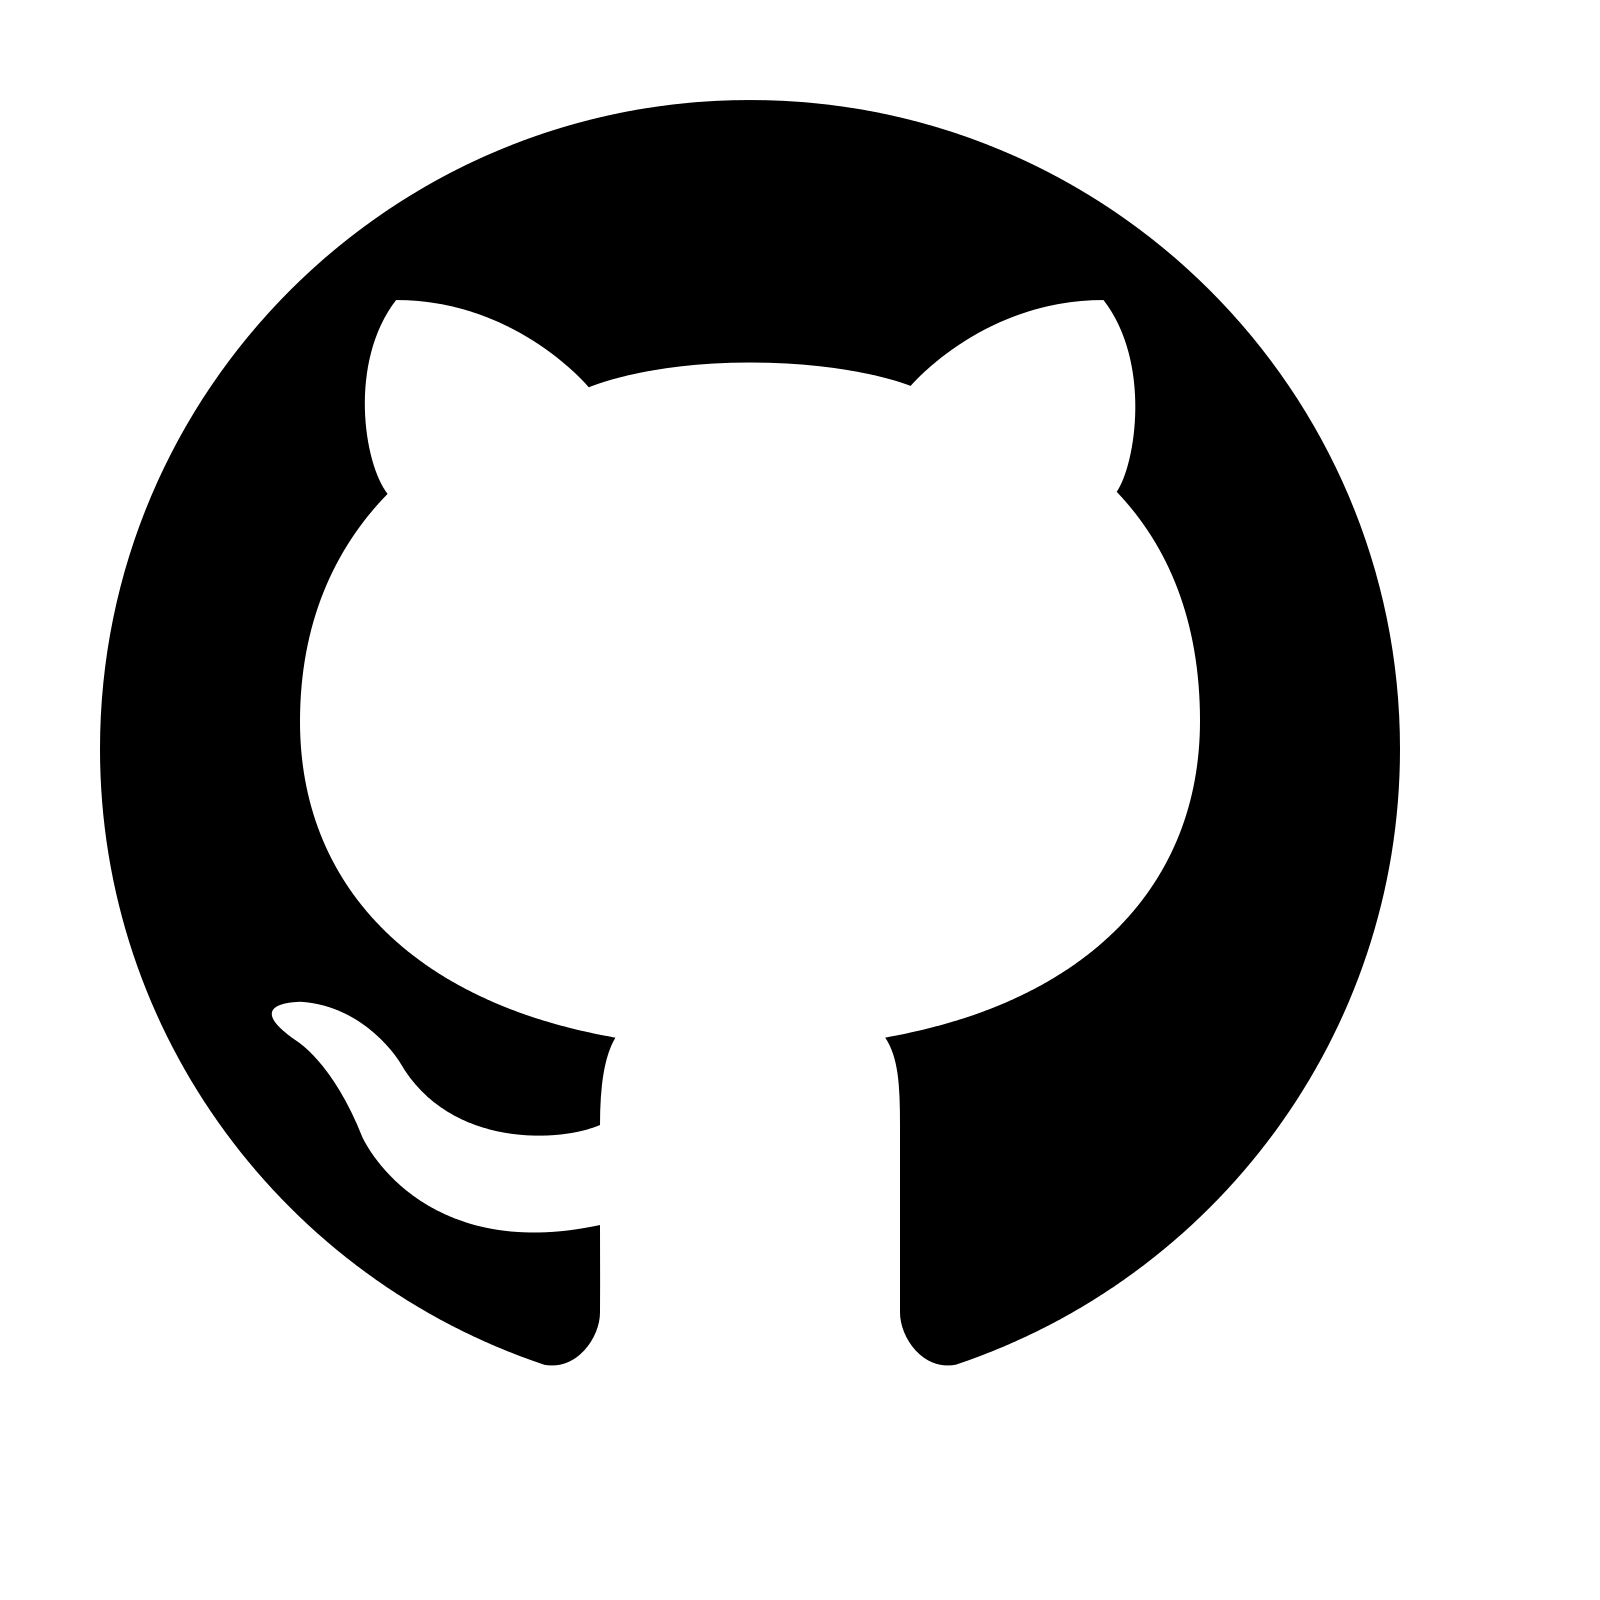
\includegraphics[width=0.04\textwidth]{imgs/github.png}
          \end{textblock}
      };
      %
      %
      %
      \node [align=center] at ($(current page.north)+(-4,-0.3\textwidth)$) (fast) {\large{Fast}};
      \draw[ultra thick,->] (fast.south) .. controls ($(fast.south)+(0,-0.6)$) .. ($(fast.south)+(0.8,-1)$);
      \node [text width=0.3\textwidth, align=center] at ($(fast.south)+(-0.75,-0.75)$) (fastimg) {
\includegraphics[width=30pt]{imgs/strong.png}};
      %
      %
      %
      \node [align=center] at ($(current page.north)+(4,-0.3\textwidth)$) (generic) {\large{Generic}};
      \draw[ultra thick,->] (generic.south) .. controls ($(generic.south)+(0,-0.6)$) .. ($(generic.south)+(-0.8,-1)$);
      \node [text width=0.3\textwidth,align=center,xscale=-1] at ($(generic.south)+(0.75,-0.75)$) (genericimg) {
\includegraphics[width=30pt]{imgs/strong.png}};
      %
      %
      %
      \node [align=center] at ($(current page.north)+(0,-0.75\textwidth)$) (works) {
          Allows \emphtwo{user-defined} \\ $\datafunc(\cdot)$ and $\regfunc(\cdot)$
      };
      \draw[ultra thick,->] (works.north) -- ($(works.north)+(0,1.9)$);
      \node [text width=0.3\textwidth, align=center] at ($(works.north)+(0.8,0.8)$) (worksimg) {
\includegraphics[width=30pt]{imgs/party.png}};
  \end{tikzpicture}
\end{frame}

\begin{frame}{The secret sauce}
  \begin{tikzpicture}[remember picture,overlay]
      \node<+-> [text width=.3\textwidth] at (current page.center) (bnb) {
          \begin{blockthree}{}
              \centering
              \textbf{Branch-and-Bound}
          \end{blockthree}
      };
      \onslide<+-> {
          \node [text width=.3\textwidth] at ($(current page.center)+(-3,+2.5)$) (cdsolver) {
              \begin{blocksix}{}
                  \centering
                  \textbf{Coordinate descent bounding solver}
              \end{blocksix}
          };
          \draw[ultra thick,->] (cdsolver.south) .. controls ($(cdsolver.south)+(0,-0.5)$) .. ($(bnb.north west)+(0,-0.25)$) node[midway,fill=white,draw=black,ultra thick] {\scriptsize{Scalability}};
      }
      \onslide<+-> {
          \node [text width=.3\textwidth] at ($(current page.center)+(-3,-2.25)$) (screening) {
              \begin{blocksix}{}
                  \centering
                  \textbf{Screening}
              \end{blocksix}
          };
          \draw[ultra thick,->] ($(screening.north)+(0,-0.25)$) .. controls ($(screening.north)+(0,+0.5)$) .. (bnb.south west) node[midway,fill=white,draw=black,ultra thick] {\scriptsize{Reduced bounding time}};
      }
      \onslide<+-> {
          \node [text width=.3\textwidth] at ($(current page.center)+(+3,+2.5)$) (nodescreening) {
              \begin{blocksix}{}
                  \centering
                  \textbf{Mixed BFD/DFS exploration}
              \end{blocksix}
          };
          \draw[ultra thick,->] (nodescreening.south) .. controls ($(nodescreening.south)+(0,-0.5)$) .. ($(bnb.north east)+(0,-0.25)$) node[midway,fill=white,draw=black,ultra thick] {\scriptsize{Quality of bounds}};
      }
      \onslide<+-> {
          \node [text width=.3\textwidth] at ($(current page.center)+(+3,-2.25)$) (exploration) {
              \begin{blocksix}{}
                  \centering
                  \textbf{Node-screening}
              \end{blocksix}
          };
          \draw[ultra thick,->] ($(exploration.north)+(0,-0.25)$) .. controls ($(exploration.north)+(0,+0.5)$) .. (bnb.south east) node[midway,fill=white,draw=black,ultra thick] {\scriptsize{Less processed nodes}};
      }
  \end{tikzpicture}
\end{frame}

\begin{frame}{Numerical results}
    \begin{tikzpicture}[remember picture,overlay]
        \node [text width=.45\textwidth] at ($(current page.north)+(0,-0.175\textheight)$) (problem) {
            \begin{blockthree}{}
                \centering
                \small
                $\min_{\pv} \ \datafunc(\pv) + \reg \norm{\pv}{0} + \regfunc(\pv)$
            \end{blockthree}
        };
        %
        %
        %
        \node<+-> [text width=.7\textwidth] at ($(current page.north)+(2.3,-0.34\textheight)$) (data) {
          \begin{itemize}[nosep]
            \item[\textbf{Dataset}] : Sparse regression
            \item[\textbf{F($\cdot$)}] : Least-squares loss
            \item[\textbf{G($\cdot$)}] : Bound constraints
            \item[$\boldsymbol{\lambda}$] : Set statistically
          \end{itemize}
        };
        \onslide<+-> {
          \begin{scope}[shift={(1,-3)}]
            \begin{axis}[
              mlineplot,
              width = 0.7\textwidth,
              height = 5cm,
              xmode = log,
              xmin = 0.05,
              xmax = 5000,
              ymax = 1.1,
              xlabel = Time (seconds),
              ylabel = Prop. solved,
              legend style={at={(1.03,0.5)},anchor=west}
            ]

            \addplot[ultra thick, smooth, color=RoyalBlue2,visible on=<3->] %
            table[x=times,y=Scip,col sep=comma]{data/perfprofiles_medium_Leastsquares_Bigm_3600.csv};
            \only<3-> {
              \addlegendentry{Scip};
            }

            \addplot[ultra thick, smooth, color=SkyBlue2,visible on=<3->] %
            table[x=times,y=Cplex,col sep=comma]{data/perfprofiles_medium_Leastsquares_Bigm_3600.csv};
            \only<3-> {
              \addlegendentry{Cplex};
            }

            \addplot[ultra thick, smooth, color=PaleGreen3,visible on=<3->] %
            table[x=times,y=Mosek,col sep=comma]{data/perfprofiles_medium_Leastsquares_Bigm_3600.csv};
            \only<3-> {
              \addlegendentry{Mosek};
            }

            \addplot[ultra thick, smooth, color=DarkGoldenrod1,visible on=<4->] %
            table[x=times,y=L0Bnb,col sep=comma]{data/perfprofiles_medium_Leastsquares_Bigm_3600.csv};
            \only<4-> {
              \addlegendentry{H. Hazimeh (2022)};
            }

            \addplot[ultra thick, smooth, color=OrangeRed1,visible on=<4->] %
            table[x=times,y=SBnb,col sep=comma]{data/perfprofiles_medium_Leastsquares_Bigm_3600.csv};
            \only<4-> {
              \addlegendentry{S. Bourguinon (2022)};
            }

            \addplot[ultra thick, smooth, color=Firebrick4,visible on=<5->] %
            table[x=times,y=El0ps,col sep=comma]{data/perfprofiles_medium_Leastsquares_Bigm_3600.csv};
            \only<5-> {
              \addlegendentry{\textbf{El0ps}};
            }
            \end{axis}
          \end{scope}
        }
      \end{tikzpicture}
\end{frame}

\begin{frame}{Numerical results}
  \begin{tikzpicture}[remember picture,overlay]
      \node [text width=.45\textwidth] at ($(current page.north)+(0,-0.175\textheight)$) (problem) {
          \begin{blockthree}{}
              \centering
              \small
              $\min_{\pv} \ \datafunc(\pv) + \reg \norm{\pv}{0} + \regfunc(\pv)$
          \end{blockthree}
      };
      %
      %
      %
      \node<+-> [text width=.7\textwidth] at ($(current page.north)+(2.3,-0.34\textheight)$) (data) {
        \begin{itemize}[nosep]
          \item[\textbf{Dataset}] : Sparse regression
          \item[\textbf{F($\cdot$)}] : Least-squares loss
          \item[\textbf{G($\cdot$)}] : \emphthree{\textbf{$\ell_2$-norm}}
          \item[$\boldsymbol{\lambda}$] : Set statistically
        \end{itemize}
      };
      \onslide<+-> {
        \begin{scope}[shift={(1,-3)}]
          \begin{axis}[
            mlineplot,
            width = 0.7\textwidth,
            height = 5cm,
            xmode = log,
            xmin = 0.05,
            xmax = 5000,
            ymax = 1.1,
            xlabel = Time (seconds),
            ylabel = Prop. solved,
            legend style={at={(1.03,0.5)},anchor=west}
          ]

          \addplot[ultra thick, smooth, color=RoyalBlue2,visible on=<2->] %
          table[x=times,y=Scip,col sep=comma]{data/perfprofiles_medium_Leastsquares_BigmL2norm_3600.csv};
          \only<2-> {
            \addlegendentry{\soutthick{Scip}};
          }

          \addplot[ultra thick, smooth, color=SkyBlue2,visible on=<2->] %
          table[x=times,y=Cplex,col sep=comma]{data/perfprofiles_medium_Leastsquares_BigmL2norm_3600.csv};
          \only<2-> {
            \addlegendentry{Cplex};
          }

          \addplot[ultra thick, smooth, color=PaleGreen3,visible on=<2->] %
          table[x=times,y=Mosek,col sep=comma]{data/perfprofiles_medium_Leastsquares_BigmL2norm_3600.csv};
          \only<2-> {
            \addlegendentry{Mosek};
          }

          \addplot[ultra thick, smooth, color=DarkGoldenrod1,visible on=<2->] %
          table[x=times,y=L0Bnb,col sep=comma]{data/perfprofiles_medium_Leastsquares_BigmL2norm_3600.csv};
          \only<2-> {
            \addlegendentry{H. Hazimeh (2022)};
          }

          \addplot[ultra thick, smooth, color=OrangeRed1,visible on=<2->] %
          table[x=times,y=SBnb,col sep=comma]{data/perfprofiles_medium_Leastsquares_BigmL2norm_3600.csv};
          \only<2-> {
            \addlegendentry{\soutthick{S. Bourguinon (2022)}};
          }

          \addplot[ultra thick, smooth, color=Firebrick4,visible on=<2->] %
          table[x=times,y=El0ps,col sep=comma]{data/perfprofiles_medium_Leastsquares_BigmL2norm_3600.csv};
          \only<2-> {
            \addlegendentry{\textbf{El0ps}};
          }
          \end{axis}
        \end{scope}
      }
    \end{tikzpicture}
\end{frame}

\begin{frame}{Numerical results}
    \begin{tikzpicture}[remember picture,overlay]
        \node [text width=.45\textwidth] at ($(current page.north)+(0,-0.175\textheight)$) (problem) {
            \begin{blockthree}{}
                \centering
                \small
                $\min_{\pv} \ \datafunc(\pv) + \reg \norm{\pv}{0} + \regfunc(\pv)$
            \end{blockthree}
        };
        %
        %
        %
        \node<+-> [text width=.7\textwidth] at ($(current page.north)+(2.3,-0.34\textheight)$) (data) {
          \begin{itemize}[nosep]
            \item[\textbf{Dataset}] : Sparse \textbf{\emphthree{classification}}
            \item[\textbf{F($\cdot$)}] : \textbf{\emphthree{Logistic loss}}
            \item[\textbf{G($\cdot$)}] : Bound constraints
            \item[$\boldsymbol{\lambda}$] : Set statistically
          \end{itemize}
        };
        \onslide<+-> {
          \begin{scope}[shift={(1,-3)}]
            \begin{axis}[
              mlineplot,
              width = 0.7\textwidth,
              height = 5cm,
              xmode = log,
              xmin = 0.05,
              xmax = 5000,
              ymax = 1.1,
              xlabel = Time (seconds),
              ylabel = Prop. solved,
              legend style={at={(1.03,0.5)},anchor=west}
            ]

            \addplot[ultra thick, smooth, color=RoyalBlue2,visible on=<2->] %
            table[x=times,y=Scip,col sep=comma]{data/perfprofiles_medium_Logistic_Bigm_3600.csv};
            \only<2-> {
              \addlegendentry{\soutthick{Scip}};
            }

            \addplot[ultra thick, smooth, color=SkyBlue2,visible on=<2->] %
            table[x=times,y=Cplex,col sep=comma]{data/perfprofiles_medium_Logistic_Bigm_3600.csv};
            \only<2-> {
              \addlegendentry{\soutthick{Cplex}};
            }

            \addplot[ultra thick, smooth, color=PaleGreen3,visible on=<2->] %
            table[x=times,y=Mosek,col sep=comma]{data/perfprofiles_medium_Logistic_Bigm_3600.csv};
            \only<2-> {
              \addlegendentry{Mosek};
            }

            \addplot[ultra thick, smooth, color=DarkGoldenrod1,visible on=<2->] %
            table[x=times,y=L0Bnb,col sep=comma]{data/perfprofiles_medium_Logistic_Bigm_3600.csv};
            \only<2-> {
              \addlegendentry{\soutthick{H. Hazimeh (2022)}};
            }

            \addplot[ultra thick, smooth, color=OrangeRed1,visible on=<2->] %
            table[x=times,y=SBnb,col sep=comma]{data/perfprofiles_medium_Logistic_Bigm_3600.csv};
            \only<2-> {
              \addlegendentry{\soutthick{S. Bourguinon (2022)}};
            }

            \addplot[ultra thick, smooth, color=Firebrick4,visible on=<2->] %
            table[x=times,y=El0ps,col sep=comma]{data/perfprofiles_medium_Logistic_Bigm_3600.csv};
            \only<2-> {
              \addlegendentry{\textbf{El0ps}};
            }
              
            \end{axis}
          \end{scope}
        }
  \end{tikzpicture}
\end{frame}

% \begin{frame}{Numerical results}
%   \begin{tikzpicture}[remember picture,overlay]
%     \node [text width=.45\textwidth] at ($(current page.north)+(0,-0.175\textheight)$) (problem) {
%     \begin{blockthree}{}
%         \centering
%         \small
%         $\min_{\pv} \ \datafunc(\pv) + \reg \norm{\pv}{0} + \regfunc(\pv)$
%     \end{blockthree}
%     };
%     %
%     %
%     %
%     \node<+-> [text width=.7\textwidth] at ($(current page.north)+(2.3,-0.34\textheight)$) (data) {
%       \begin{itemize}[nosep]
%         \item[\textbf{Dataset}] : Sparse regression
%         \item[\textbf{F($\cdot$)}] : Least-squares loss
%         \item[\textbf{G($\cdot$)}] : Bound constraints
%         \item[$\boldsymbol{\lambda}$] : \textbf{\emphthree{From $\regmax$ to $\reg_{\min}$}}
%       \end{itemize}
%     };
%     %
%     %
%     %
%     \onslide<+-> {
%       \begin{scope}[shift={(1,-3)}]
%         \begin{axis}[
%           mlineplot,
%           width = 0.7\textwidth,
%           height = 5cm,
%           xmode = log,
%           ymode = log,
%           x dir = reverse,
%           ymin = 0.00007,
%           ymax = 8000,
%           xmin = 0.009,
%           xmax = 1.2,
%           xlabel = {$\reg/\regmax$},
%           ylabel = Solve time,
%           ytick = {0.01,1,100},
%           legend style={at={(1.03,0.5)},anchor=west}
%         ]

%         \addplot[ultra thick, smooth, color=RoyalBlue2,visible on=<2->] %
%         table[x=lambdaratio,y=Scip,col sep=comma]{data/regpath_Leastsquares_Bigm_1.0_0.01_600.csv};
%         \only<2-> {
%           \addlegendentry{Scip};
%         }

%         \addplot[ultra thick, smooth, color=SkyBlue2,visible on=<2->] %
%         table[x=lambdaratio,y=Cplex,col sep=comma]{data/regpath_Leastsquares_Bigm_1.0_0.01_600.csv};
%         \only<2-> {
%           \addlegendentry{Cplex};
%         }

%         \addplot[ultra thick, smooth, color=PaleGreen3,visible on=<2->] %
%         table[x=lambdaratio,y=Mosek,col sep=comma]{data/regpath_Leastsquares_Bigm_1.0_0.01_600.csv};
%         \only<2-> {
%           \addlegendentry{Mosek};
%         }

%         \addplot[ultra thick, smooth, color=DarkGoldenrod1,visible on=<2->] %
%         table[x=lambdaratio,y=L0Bnb,col sep=comma]{data/regpath_Leastsquares_Bigm_1.0_0.01_600.csv};
%         \only<2-> {
%           \addlegendentry{H. Hazimeh (2022)};
%         }

%         \addplot[ultra thick, smooth, color=OrangeRed1,visible on=<2->] %
%         table[x=lambdaratio,y=SBnb,col sep=comma]{data/regpath_Leastsquares_Bigm_1.0_0.01_600.csv};
%         \only<2-> {
%           \addlegendentry{S. Bourguinon (2022)};
%         }

%         \addplot[ultra thick, smooth, color=Firebrick4, visible on=<2->] %
%         table[x=lambdaratio,y=El0ps,col sep=comma]{data/regpath_Leastsquares_Bigm_1.0_0.01_600.csv};
%         \only<2-> {
%           \addlegendentry{\textbf{El0ps}};
%         }

%         \addplot[ultra thick, smooth, color=black, densely dashed, visible on=<2->] %
%         table[x=lambdaratio,y=Maxtime,col sep=comma]{data/regpath_Leastsquares_Bigm_1.0_0.01_600.csv};
          
%         \end{axis}
%       \end{scope}
%     }
%   \end{tikzpicture}
% \end{frame}

\begin{frame}{Conclusion}
  \begin{tikzpicture}[remember picture,overlay]
    \node [text width=.45\textwidth] at ($(current page.north)+(0,-0.25\textheight)$) (problem) {
        \begin{blockthree}{$\ell_0$-penalized problem}
            \centering
            $\min_{\pv} \ \datafunc(\pv) + \reg \norm{\pv}{0} + \regfunc(\pv)$
        \end{blockthree}
    };
    \onslide<+-> {
      \node [text width=\textwidth] at ($(current page.north)+(0,-0.65\textheight)$) (observations) {
        \begin{itemize}[label=$\blacktriangleright$]
          \item<+-> Generic solution method
          \begin{itemize}[label=$\bullet$]
            \item $\datafunc(\cdot)$ convex
            \item $\regfunc(\cdot)$ convex and separable
          \end{itemize}
          \item<+-> Significant gains against competitors
          \begin{itemize}[label=$\bullet$]
            \item Factor $\times10^{6}$ against off-the-shelf solvers
            \item Factor $\times10^{2}$ against specialized solvers
          \end{itemize}
          \item<+-> We do not trade \emphtwo{efficiency} for \emphtwo{flexibility}
          \begin{itemize}[label=$\bullet$]
            \item Handle broader practical cases
            \item Address more challenging instances
          \end{itemize}
        \end{itemize}
      };
    }
  \end{tikzpicture}
\end{frame}
\begin{frame}[standout]
    \begin{tikzpicture}[remember picture,overlay]
        \node at ($(current page.north)+(0,-2)$) {Question time};
        \node at ($(current page.north)+(0,-3)$) {
            
\includegraphics[width=30pt]{imgs/nerd_face.png}
        };  
        %
        %
        %
        \draw[ultra thick, fill=white] (-0.29\textwidth,-0.23\textwidth) rectangle (0.29\textwidth,-0.45\textheight);
        \node [text width=0.7\textwidth] at ($(current page.north)+(0,-0.7\textwidth)$) (repo) {
            \begin{textblock}{1}(-0.15,-0.025)
                \centering
                \LARGE{TheoGuyard/\bf{El0ps.jl}}
            \end{textblock}
            \begin{textblock}{1}(-0.19,0.055)
                \centering
                \scriptsize{\textcolor{gray}{An Exact L0-penalized Problem Solver}}
            \end{textblock}
            \begin{textblock}{1}(0.59,0.06)
                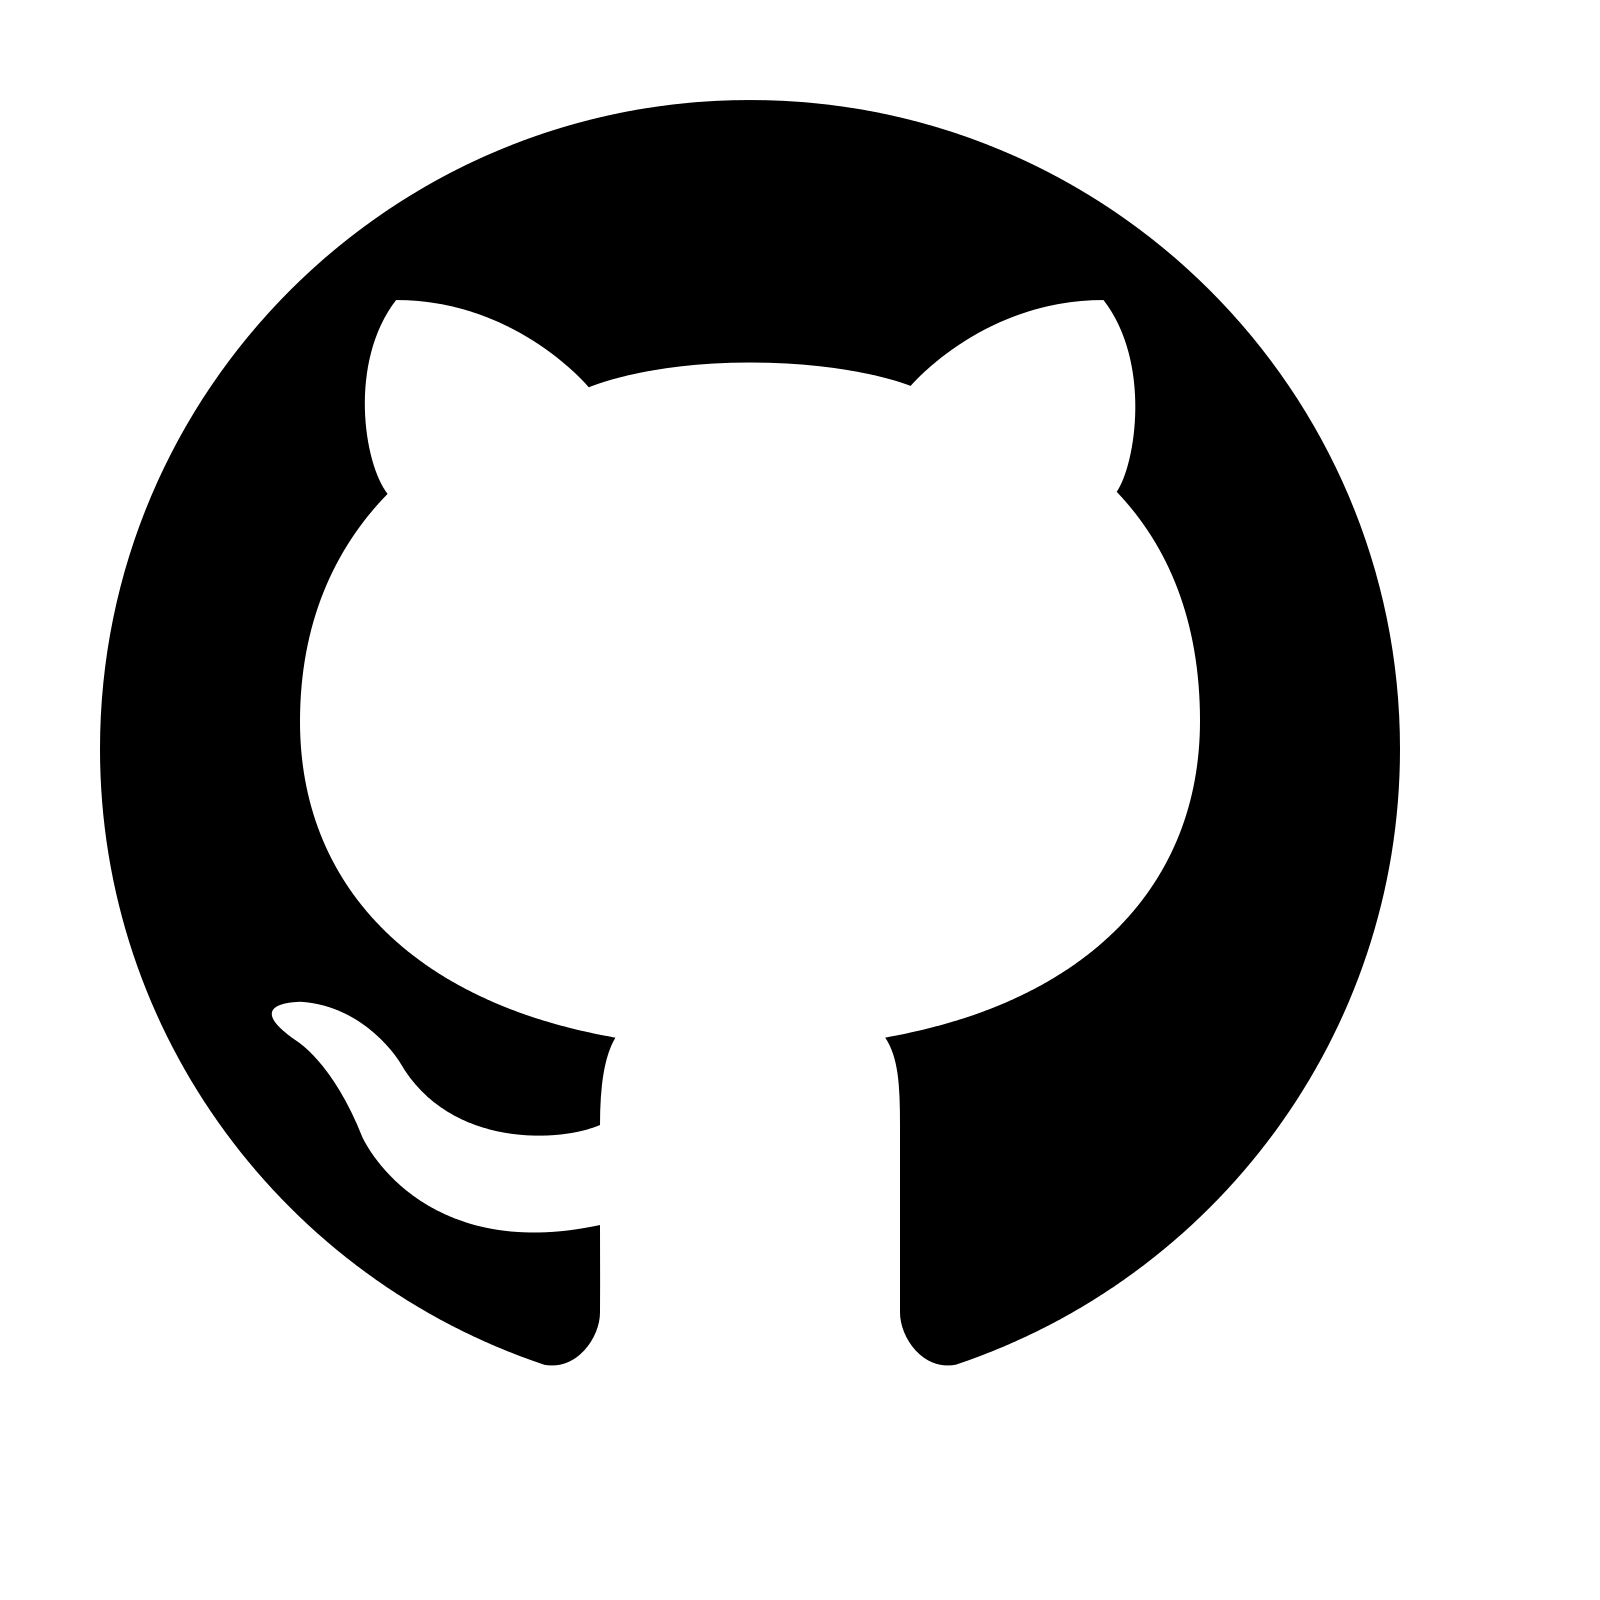
\includegraphics[width=0.04\textwidth]{imgs/github.png}
            \end{textblock}
        };
        %
        %
        %
        \node at ($(current page.north)+(0,-0.6\textwidth)$) {
            
\includegraphics[width=20pt]{imgs/point_down.png}
        };
    \end{tikzpicture}
\end{frame}


\end{document}